\section{Analysis Of The Recording}

All the important parts of the recording:

%%%Client hello:

\begin{figure}[H] % Client Hello
\center{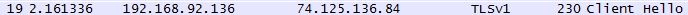
\includegraphics[width=1\linewidth]{ClientHello}}
\caption{Client Hello}
\label{fig:speciation}
\end{figure}

This is the Client Hello packet seen from wireshark. From this we can see the client's ip adress (192.168.92.136) and the server's ip adress (74.125.136.84) and that the recording used TLS instead of SSL.

\vspace{5mm}\hrule\vspace{5mm}
%---------------------

\begin{figure}[H] % TLS verson
\center{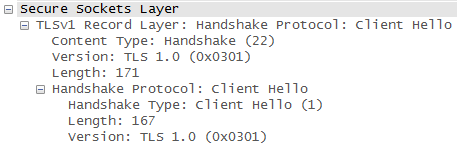
\includegraphics[width=0.8\linewidth]{TLSverson}}
\caption{TLS verson}
\label{fig:speciation}
\end{figure}

Version Number:
Client sends the version number corresponding to the highest version it supports. In this case TLS version 1.0.

\vspace{5mm}\hrule\vspace{5mm}
%---------------------

\begin{figure}[H] % Client Random
\center{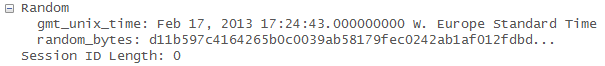
\includegraphics[width=1\linewidth]{ClientRandom}}
\caption{Client Random}
\label{fig:speciation}
\end{figure}

here the cient generates a 32 byte value consisting of a 4-byte number that contains the client’s date and time, plus a 28 byte randomly generated number that ultimately will be used with the server random value to generate a master secret. In this case we can see that the recording was done on feb 17  2013.

\vspace{5mm}\hrule\vspace{5mm}
%---------------------

\begin{figure}[H] % Client Cipher Suits
\center{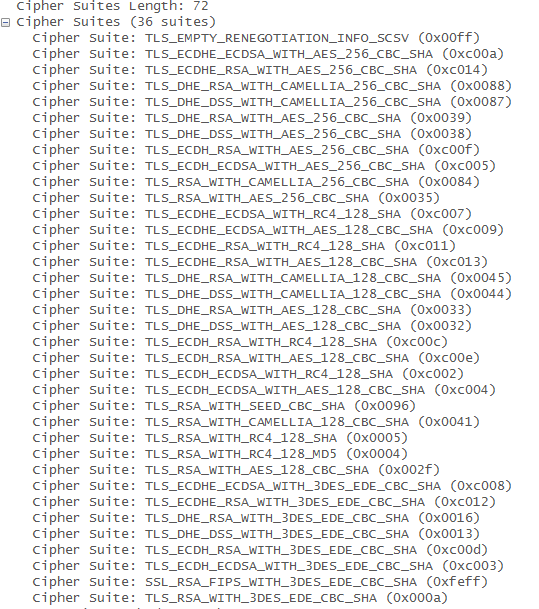
\includegraphics[width=0.8\linewidth]{ClientCipherSuits}}
\caption{Client Cipher Suits}
\label{fig:speciation}
\end{figure}

In this tab we can see that the client sends all the different cipher suits that it is compatible with. Every part of the name describes the different parts the suit is using.
Taking TLS\_RSA\_WITH\_DES\_CBC\_SHA as an example: TLS is the protocol version, RSA is the algorithm that will be used for the key exchange, DES\_CBC is the encryption algorithm (using a 56-bit key in CBC mode), and SHA is the hash function.

\vspace{5mm}\hrule\vspace{5mm}
%---------------------

\begin{figure}[H] % Client Curves
\center{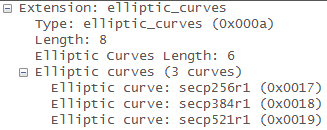
\includegraphics[width=0.5\linewidth]{ClientCurves}}
\caption{Client Curves}
\label{fig:speciation}
\end{figure}

In this recording we can also see that elliptic curves are in use, and here the client sends three different curves that the client supports.

\vspace{5mm}\hrule\vspace{5mm}
%---------------------

\begin{figure}[H] % Client EC Point Format
\center{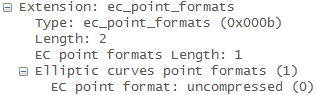
\includegraphics[width=0.6\linewidth]{ClientECPointFormat}}
\caption{Client EC Point Format}
\label{fig:speciation}
\end{figure}

The client EC Point Formats is a list of the point formats a client is able to parse, which the client is required to send with the ClientHello message when it suggests the use of elliptic curves as is the case when using the Elliptic Curve variety of an algorithm such as Diffie-Hellman.

\vspace{5mm}\hrule\vspace{5mm}
%---------------------

%%% Server hello:

\begin{figure}[H] % Server Hello
\center{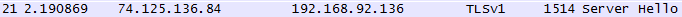
\includegraphics[width=1\linewidth]{ServerHello}}
\caption{Server Hello}
\label{fig:speciation}
\end{figure}

This is the server hello packet seen from wireshark. 

\vspace{5mm}\hrule\vspace{5mm}
%---------------------

\begin{figure}[H] % ServerTLSVerson
\center{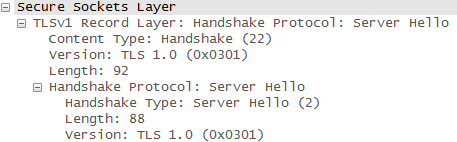
\includegraphics[width=0.8\linewidth]{ServerTLSVerson}}
\caption{Server TLS Verson}
\label{fig:speciation}
\end{figure}

The server sends the highest version number supported by BOTH sides.

\vspace{5mm}\hrule\vspace{5mm}
%---------------------

\begin{figure}[H] % Server Random
\center{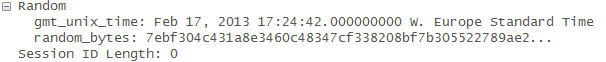
\includegraphics[width=1\linewidth]{ServerRandom}}
\caption{Server Random}
\label{fig:speciation}
\end{figure}

Here the server creates a random number the same way the client did earlier.

\vspace{5mm}\hrule\vspace{5mm}
%---------------------

\begin{figure}[H] % Server Cipher Suite
\center{
\includegraphics[width=0.8\linewidth]{ServerCipherSuite}}
\caption{Server Cipher Suite}
\label{fig:speciation}
\end{figure}

The server will choose the strongest cipher that BOTH the client and server support. In this case its TLS\_ECDHE\_RSA\_WITH\_RC4\_128\_SHA (0xc011).
If no cipher is supported by both the client and server, the session is ended with a “Handshake Failure” alert.

\vspace{5mm}\hrule\vspace{5mm}
%---------------------

\begin{figure}[H] % Server EC Point Formats
\center{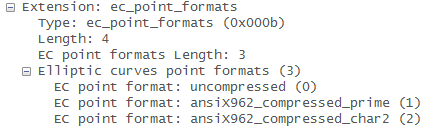
\includegraphics[width=0.8\linewidth]{ServerECPointFormats}}
\caption{Server EC Point Formats}
\label{fig:speciation}
\end{figure}

When the server has received a ClientHello containing a list of elliptic curves and chosen a curve it wishes to use, it's required to use the point format suggested by the client to describe the point on the curve it wishes to use, as well as the curve it wishes to use.

\vspace{5mm}\hrule\vspace{5mm}
%--------------------- %%Certificate:

\begin{figure}[H] % Certificate
\center{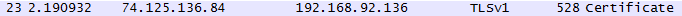
\includegraphics[width=1\linewidth]{Certificate}}
\caption{Certificate}
\label{fig:speciation}
\end{figure}

The server now sends it's Certificate to the client.

\vspace{5mm}\hrule\vspace{5mm}
%---------------------

\begin{figure}[H] % CertificateTLSverson
\center{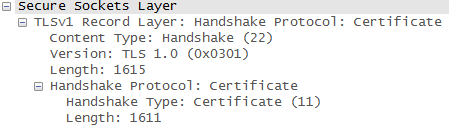
\includegraphics[width=0.8\linewidth]{CertificateTLSverson}}
\caption{Certificate TLS verson}
\label{fig:speciation}
\end{figure}



\vspace{5mm}\hrule\vspace{5mm}
%---------------------

\begin{figure}[H] % CertificateCertificates
\center{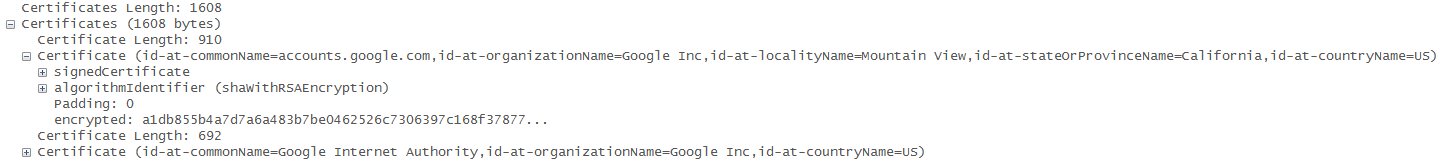
\includegraphics[width=1.2\linewidth]{CertificateCertificates}}
\caption{Certificate Certificates}
\label{fig:speciation}
\end{figure}

In this tab we can see the different certificates the servers send, and all their information (1608bytes). 
On the first line we can se the total lenght of all the certificates in the tab. we can then see the lenght of the first certificate, in the case its 910bytes. After that we see those 910bytes in data form.

\vspace{5mm}\hrule\vspace{5mm}
%---------------------

\begin{figure}[H] % Certificate EC Diffie Hellman Server Params
\center{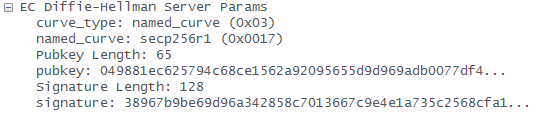
\includegraphics[width=1\linewidth]{CertificateECDiffieHellmanServerParams}}
\caption{Certificate EC Diffie Hellman Server Params}
\label{fig:speciation}
\end{figure}

Here the server sends it's choice out of the curves the client supported. In this case the server chose the secp256r1 curve. 
The server then sends the public key length, followed by the public key.
This message also contains a signature that proves possession of the private key corresponding to client's public key.

\vspace{5mm}\hrule\vspace{5mm}
%---------------------

\begin{figure}[H] % CertificateServerKeyExchange
\center{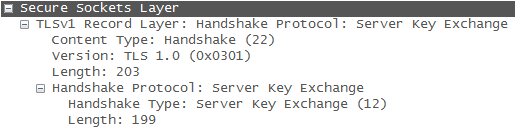
\includegraphics[width=0.8\linewidth]{CertificateServerKeyExchange}}
\caption{Certificate Server Key Exchange}
\label{fig:speciation}
\end{figure}

The server sends it's ephemeral ECDH public key to the client

\vspace{5mm}\hrule\vspace{5mm}
%---------------------

\begin{figure}[H] % Server Hello Done
\center{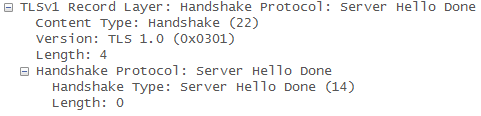
\includegraphics[width=0.8\linewidth]{ServerHelloDone}}
\caption{Server Hello Done}
\label{fig:speciation}
\end{figure}

The server has now told the client that it is done, and are now waiting for a response from the client.
%%% Client key exchange:
\vspace{5mm}\hrule\vspace{5mm}

\begin{figure}[H] % Client Key Exchange
\center{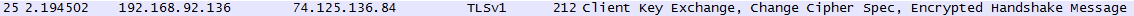
\includegraphics[width=1\linewidth]{ClientKeyExchange}}
\caption{Client Key Exchange}
\label{fig:speciation}
\end{figure}

\vspace{5mm}\hrule\vspace{5mm}
%---------------------

\begin{figure}[H] % Client Key Exchange Verson 
\center{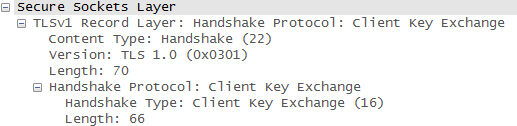
\includegraphics[width=0.8\linewidth]{ClientKeyExchangeVerson}}
\caption{Client Key Exchange Version}
\label{fig:speciation}
\end{figure}

\vspace{5mm}\hrule\vspace{5mm}
%---------------------

\begin{figure}[H] % Client Key Exchange DiffieHellman Client Params
\center{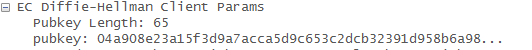
\includegraphics[width=1\linewidth]{ClientKeyExchangeDiffieHellmanClientParams}}
\caption{Client Key Exchange DiffieHellman Client Params}
\label{fig:speciation}
\end{figure}

The client sends a Client Key Exchange message after computing the premaster secret using both random values.
The premaster secret is encrypted by the public key from the server’s certificate before being transmitted to the server.
Both the client and server will compute the master secret locally and derive the session key from it.

\vspace{5mm}\hrule\vspace{5mm}
%---------------------

\begin{figure}[H] % Client Key Exchange Change Cipher
\center{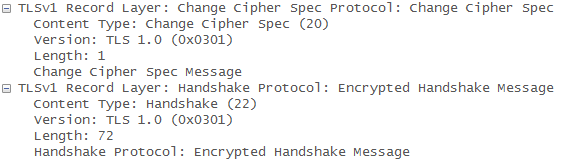
\includegraphics[width=1\linewidth]{ClientKeyExchangeChangeCipher}}
\caption{Client Key Exchange Change Cipher}
\label{fig:speciation}
\end{figure}

This message contains a change cipher spec message, and an encrypted handshake message wich contains a summary of the whole handshake.

\vspace{5mm}\hrule\vspace{5mm}
%---------------------

\begin{figure}[H] % NewSessionTicket
\center{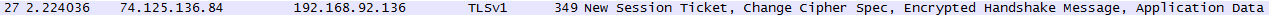
\includegraphics[width=1\linewidth]{NewSessionTicket}}
\caption{New Session Ticket}
\label{fig:speciation}
\end{figure}

The client requests to start a new session after the handshake to transfer data.

\vspace{5mm}\hrule\vspace{5mm}
%---------------------

\begin{figure}[H] % Client Session Ticket
\center{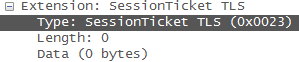
\includegraphics[width=0.6\linewidth]{ClientSessionTicket}}
\caption{Client Session Ticket}
\label{fig:speciation}
\end{figure}

\vspace{5mm}\hrule\vspace{5mm}
%---------------------

\begin{figure}[H] % ApplicationData
\center{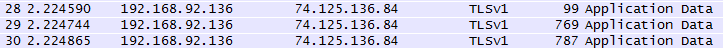
\includegraphics[width=1\linewidth]{ApplicationData}}
\caption{Application Data}
\label{fig:speciation}
\end{figure}

Data packets sent after the TLS handshake is successful.s
